\begin{defn}[Factorials]\index{factorial}
    The number of ways to arrange \(n\) objects is called \emph{\(n\)-factorial} and is calculated like so:
    \[n!=n\cdot(n-1)\cdot(n-2)\cdots2\cdot1.\]
\end{defn}

\begin{defn}[Permutations]\index{permutation}
    \emph{Permutations} represent the number of ways to select \(k\) object from \(n\) options when \emph{order does matter} and are calculated like so:
        \[_nP_k=\frac{n!}{(n-k)!}=n\cdot(n-1)\cdot(n-2)\cdots(n-k+1).\]
    We can derive this like so:\vspace{0.2\textheight}
\end{defn}

\begin{defn}[Combinations]\index{combination}
    \emph{Combinations} represent the number of ways to select \(k\) object from \(n\) options when \emph{order does not matter} and are calculated like so:
        \[_nC_k=\binom{n}{k}=\frac{n!}{k!(n-k)!}=\frac{n\cdot(n-1)\cdot(n-2)\cdots(n-k+1)}{k\cdot(k-1)\cdot(k-2)\cdots2\cdot1}.\]
    This is sometimes also called a \emph{binomial coefficients} because we either choose an option or not.
    We can derive this like so:\vspace{0.2\textheight}
\end{defn}

\clearpage

\begin{practiceprob}{Basic Calculations}
    Translate each of the following into a mathematical expression and then complete the calculation.
    \begin{enumerate}
    \setlength{\itemsep}{70pt}
        \item Pick 5 out of 7 distinct objects when order matters:
        \item Arrange 6 distinct objects:
        \item Pick 3 out of 5 distinct objects when order doesn't matter:
        \item Pick 10 out of 15 distinct objects when order matters:
        \item Arrange 17 distinct objects:
        \item Pick 7 out of 10 distinct objects when order doesn't matter:\vspace{70pt}
    \end{enumerate}
\end{practiceprob}

\begin{exposition}\index{deck of cards}\index{suit}\index{rank}
    Below is a standard deck of cards with four suits and thirteen ranks per suit.
    \begin{figure}[H]
        \centering
        % \inputtikz{deck_of_cards}
        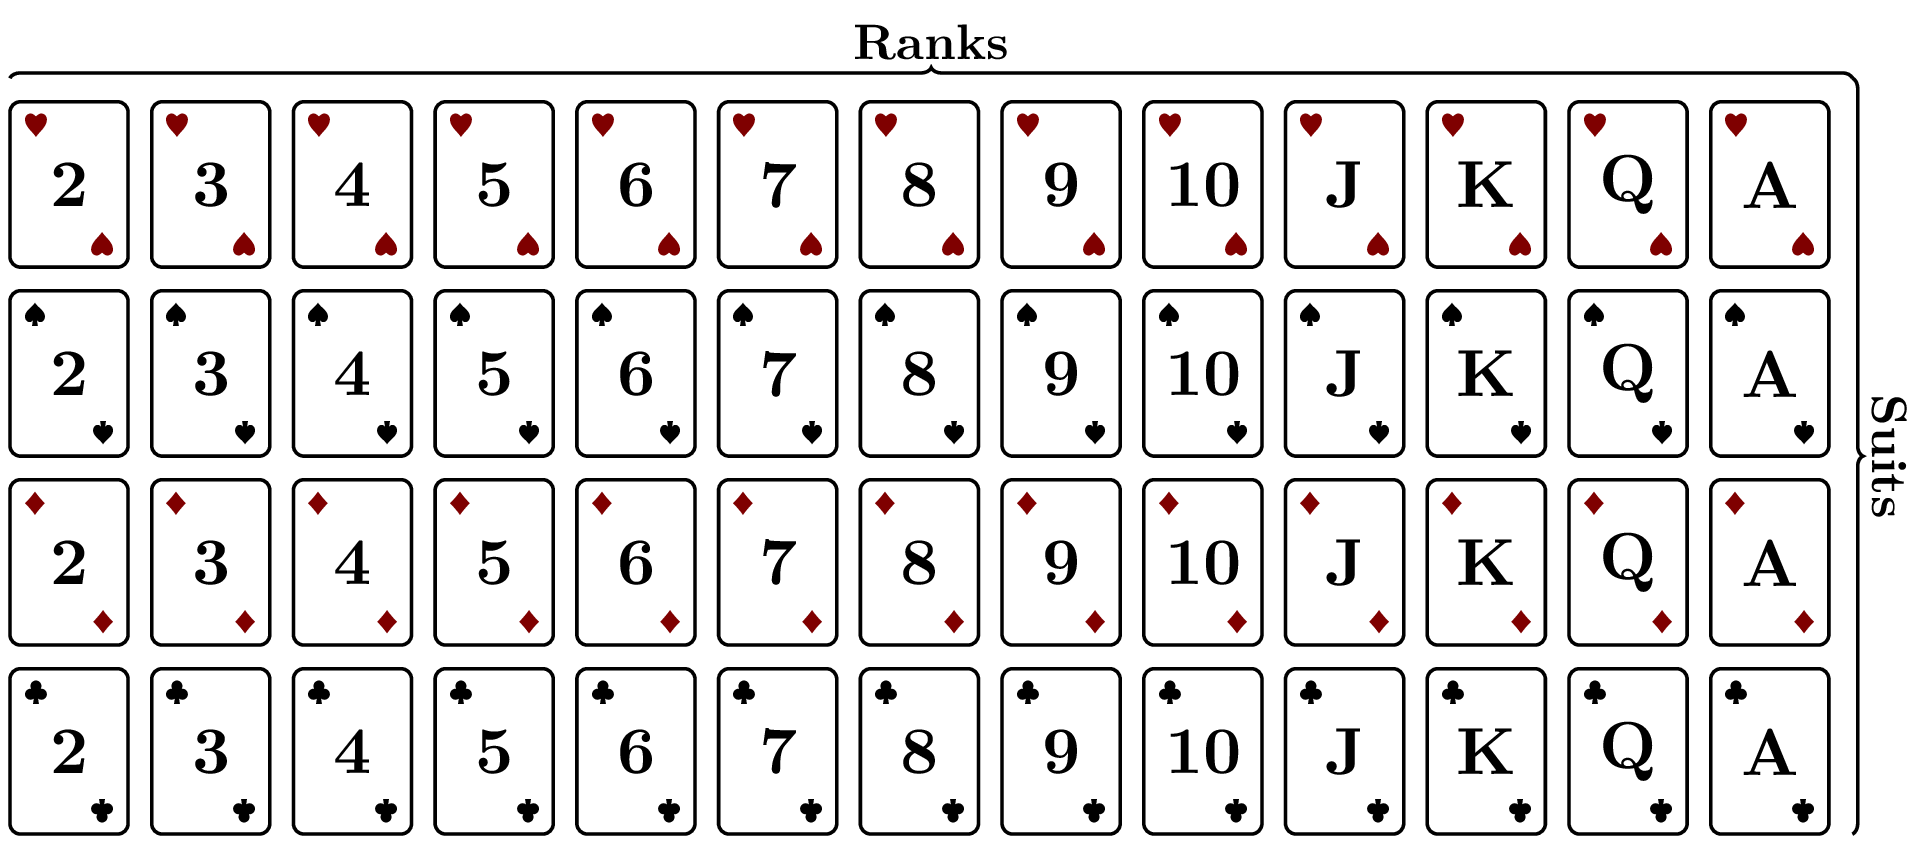
\includegraphics[scale=0.24,alt={deck of cards with four suits and thirteen ranks per suit}]{images/created/deck_of_cards.png}
        \caption{Standard Deck of Cards}
        \label{fig:card-deck}
    \end{figure}

    \noindent
    If we deal 5 cards from a standard deck, there are 3744 full houses like:
    \begin{figure}[H]
        \centering
        % \inputtikz{full_house}
        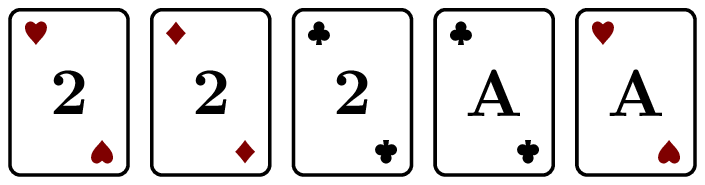
\includegraphics[scale=0.24,alt={full house card hand}]{images/created/full_house.png}
        \caption{Full House}
        \label{fig:full-house}
    \end{figure}
    We can use combinations to see why.  First \emph{make a plan} and second calculate.
    \begin{sides}[lefthand width=0.5\textwidth]
        \begin{enumerate}
            \item Pick 1 of 13 ranks for the 3 of a kind
            \item Pick 3 of 4 from that rank
            \item Pick 1 of 12 ranks for the pair
            \item Pick 2 of 4 from that rank
        \end{enumerate}
        \tcblower
        \begin{align*}
            \binom{13}{1}\binom{4}{3}\binom{12}{1}\binom{4}{2}&=13\cdot4\cdot12\cdot6\\
                &=3744\ \text{\accentcheckmark}
        \end{align*}
    \end{sides}
\end{exposition}

\begin{practiceprob}
    If we deal 5 cards from a standard deck, there are 624 four of a kinds like:
    \begin{figure}[H]
        \centering
        % \inputtikz{four_kind}
        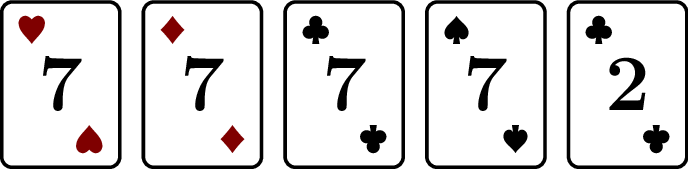
\includegraphics[scale=0.24,alt={four of a kind card hand}]{images/created/four_kind.png}
        \caption{Four of a Kind}
        \label{fig:four-kind}
    \end{figure}
    We can use combinations to see why.  First \emph{make a plan} and second calculate.
    \begin{sides}[lefthand width=0.5\textwidth]
        \begin{enumerate}
        \setlength\itemsep{10pt}
            \item 
            \item 
            \item\phantom{stuff} \vspace{10pt}
        \end{enumerate}
        \tcblower
        % \begin{align*}
        %     \binom{13}{1}\binom{4}{4}\binom{48}{1}&=13\cdot1\cdot48\\
        %         &=624\ \text{\accentcheckmark}
        % \end{align*}
    \end{sides}
\end{practiceprob}

% \clearpage

\begin{exposition}[Three of a Kind Done the Wrong]
    Now we want to know how many ways we can make a three of a kind, looking it up the answer is 54912, but why?
    \begin{figure}[H]
        \centering
        % \inputtikz{three_kind}
        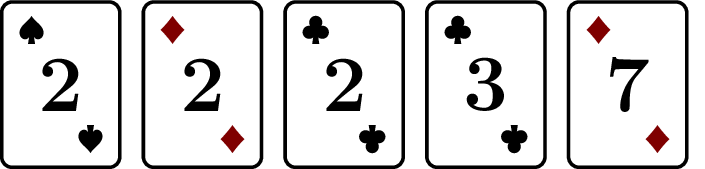
\includegraphics[scale=0.24,alt={three of a kind card hand}]{images/created/three_kind.png}
        \caption{Three of a Kind}
        \label{fig:three-kind}
    \end{figure}
    We can use combinations to see why.  First \emph{make a plan} and second calculate.
    \begin{sides}[lefthand width=0.5\textwidth]
        \begin{enumerate}
            \item Pick 1 of 13 ranks for the 3 of a kind
            \item Pick 3 of 4 from that rank
            \item Pick 2 of 49 other cards
        \end{enumerate}
        \tcblower
        \begin{align*}
            \binom{13}{1}\binom{4}{3}\binom{49}{2}&=13\cdot4\cdot\frac{49\cdot48}{2}\\
                &=61152\ \text{\accentXbrush}
        \end{align*}
    \end{sides}
    So, what did we do wrong?
    \vspace{5\baselineskip}
\end{exposition}

\begin{practiceprob}[Three of a Kind Done the Right]
    Let's look at figure \ref{fig:three-kind} again, and lets make a better plan to show there are 54912 possible three of a kinds. First \emph{make a plan} and second calculate.
    \begin{sides}[lefthand width=0.5\textwidth]
        \begin{enumerate}
        \setlength\itemsep{22pt}
            \item
            \item
            \item
            \item
            \item\phantom{stuff}\vspace{22pt}
        \end{enumerate}
        \tcblower
    \end{sides}
\end{practiceprob}

\begin{practiceprob}
    There are 123552 different ways to be dealt two pair.
    \begin{figure}[H]
        \centering
        % \inputtikz{two_pair}
        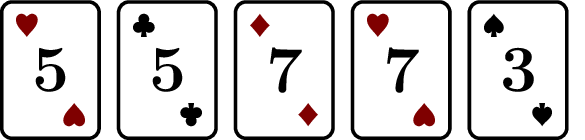
\includegraphics[scale=0.24,alt={two pair card hand}]{images/created/two_pair.png}
        \caption{Two Pair}
        \label{fig:two-pair}
    \end{figure}
    We can use combinations to see why.  First \emph{make a plan} and second calculate.
    \begin{sides}[lefthand width=0.5\textwidth]
        \begin{enumerate}
        \setlength\itemsep{22pt}
            \item 
            \item
            \item
            \item
            \item\phantom{stuff}\vspace{22pt}
        \end{enumerate}
        \tcblower
    \end{sides}
\end{practiceprob}

\begin{practiceprob}
    There are 2533180 different ways to be dealt a hand with at least one red card.
    \begin{figure}[H]
        \centering
        % \inputtikz{reds}
        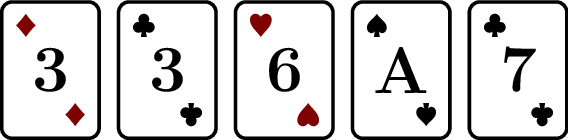
\includegraphics[scale=0.24,alt={card ahnd with one or more red cards}]{images/created/reds.png}
        \caption{One or More Red Cards}
        \label{fig:more-reds}
    \end{figure}
    We can use combinations to see why.  First \emph{make a plan} and second calculate. (This one is tricky.)
    \begin{sides}[lefthand width=0.5\textwidth]
        \begin{enumerate}
        \setlength\itemsep{2pt}
            \item 
            \item
            \item\phantom{stuff}\vspace{2pt}
        \end{enumerate}
        \tcblower
    \end{sides}
\end{practiceprob}

% Triangle, Formula, Binomial, Multinomial Coefficients
    
\begin{thm}[Pascal's Formula]\index{Pascal's Formula}
    Given positive integers \(0<k<n\), 
    \begin{equation}\label{eq:pascal}
        \binom{n+1}{k+1}=\binom{n}{k}+\binom{n}{k+1}.
    \end{equation}
\end{thm}

\begin{exposition}[Pascal's Triangle]\index{Pascal's Triangle}
    Using Pascal's Formula (equation \ref{eq:pascal}) we can create Pascal's Arithmetic Triangle:
    \begin{figure}[H]
        \centering
        % \inputtikz{pascals_triangle}
        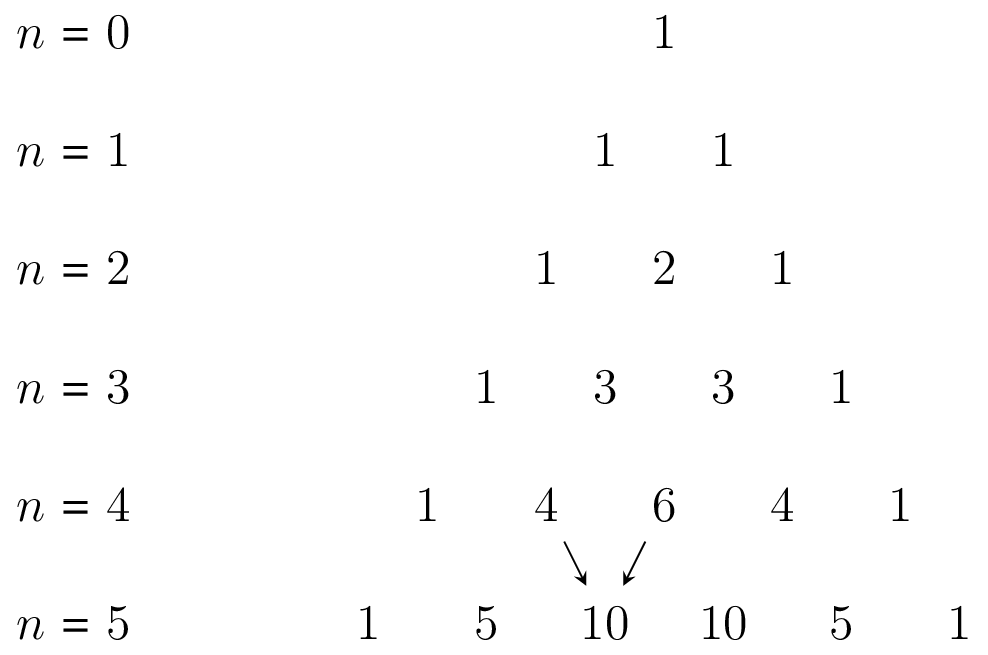
\includegraphics[scale=0.24,alt={the first six rows of pascal's triangle}]{images/created/pascals_triangle.png}
        \caption{Pascal's Triangle}
        \label{fig:pascal-tirangle}
    \end{figure}
    which lists the \emph{binomial coefficients} for each value of \(n\).
\end{exposition}

\begin{thm}[Binomial Theorem]\index{binomial theorem}
    Given a positive integer \(n\) and variables \(a\) and \(b\):
    \begin{align}\label{eq:binom}
        (a+b)^n&=(a+b)(a+b)\cdots(a+b)\\
            &=a^n+\binom{n}{1}a^{n-1}b+\binom{n}{2}a^{n-2}b^2+\cdots+\binom{n}{n-1}ab^{n-1}+b^n\\
            &=\sum_{k=0}^{n}\binom{n}{k}a^{n-k}b^k
    \end{align}
\end{thm}

\begin{practiceprob}[Sum of Pascal Rows]
    Show that the sum of the coefficients in row \(n\) of Pascal's Triangle is \(2^n\).  (Hint: \((1+1)=2\))
    \vspace{0.25\textheight}
\end{practiceprob}


% \clearpage

\begin{practiceprob}
    In the product \[(x+y+z)^{5}=(x+y+z)(x+y+z)(x+y+z)(x+y+z)(x+y+z)\]
    the coefficient for the term \(x^2yz^2\) is 30. We can use combinations to see why.  First \emph{make a plan} and second calculate.
    \begin{sides}[lefthand width=0.5\textwidth]
        \begin{enumerate}
        \setlength\itemsep{25pt}
            \item 
            \item
            \item\phantom{stuff}\vspace{25pt}
        \end{enumerate}
        \tcblower
    \end{sides}
\end{practiceprob}

\begin{practiceprob}
    There are 34650 distinct ways to rearrange the 11 letters in the word Mississippi. We can use combinations to see why.  First \emph{make a plan} and second calculate.
    \begin{sides}[lefthand width=0.5\textwidth]
        \begin{enumerate}
        \setlength\itemsep{25pt}
            \item 
            \item
            \item
            \item\phantom{stuff}\vspace{25pt}
        \end{enumerate}
        \tcblower
    \end{sides}
\end{practiceprob}

\begin{defn}[Multinomial Coefficients] \index{multinomial coefficients}
    There are two ways to think of a \emph{multinomial coefficient}. Given \(k\) different types of objects with \(n_i\) of each type, a \emph{multinomial coefficient} where \(\sum n_i=n\), represents the number of ways to arrange all the objects.
    \begin{center}
        OR
    \end{center}
    Given \(n\) copies of a set each with the same \(k\) distinct objects, a \emph{multinomial coefficient} where \(\sum n_i=n\), represents the number of ways to select \(n_i\) copies of object type \(i\).\vspace{\baselineskip}

    Either way it is calculated with:
    
    \[\binom{n}{n_1,n_2,\ldots,n_k}=\frac{n!}{n_1!n_2!\cdots n_k!}\]
    
\end{defn}


% \clearpage

\begin{thm}[Combinations with Repetition]\label{thm:comb_rep}\index{combinations with repetition}
    If we have to make \(r\) choices from \(n\) options, order does not matter, and we are allowed to select the same option more than once, then this is a \emph{combination with repetition}.  the number of ways we can do this is:
    \[\binom{r+n-1}{n-1}=\binom{r+n-1}{r}.\]
\end{thm}

\begin{exposition}
    Suppose you program a machine that scoops ice cream.  It can only follow two commands, scoop to take a scoop of whatever ice cream it is above and move to move to the next flavor.  Assuming you get three scoops of ice cream and there are five flavors, the commands for the robot could look like:

    \begin{minted}{python}
    def serving([m,m,s,m,s,m,s]):
        move arm
        move arm
        scoop ice cream
        move arm
        scoop ice cream
        move arm
        scoop ice cream
        return ice cream
    \end{minted}        

    \begin{itemize}
        \item Why are there only four move commands if there are five flavors?
        \item If \(r=3\) is the number of scoops and \(n=5\) is the number of flavors, why does it make since to use \(r+n-1=7\) like in theorem \ref{thm:comb_rep}?
    \end{itemize}

    One way of looking at this is that 
    \[
        \binom{r+n-1}{r}=\binom{7}{3}=35
    \]
    is the number of ways we can place the three scoop commands in the seven lines of code, and then put the move commands on the remaining empty lines:
    \begin{minted}{python}
    def serving([s,s,_,_,s,_,_]):
        scoop ice cream
        scoop ice cream
        _______________ 
        _______________ 
        scoop ice cream
        _______________ 
        _______________ 
        return ice cream
    \end{minted}
\end{exposition}

% \clearpage

\begin{exposition}
    Another way to think of theorem \ref{thm:comb_rep} is to ask in how many ways could you divide a row of identical objects into individual groups (we allow some groups to be empty).  For example we can split a group of 10 zombies into 4 smaller groups like so
    \begin{center}
        % \inputtikz{zombie_walls1}
        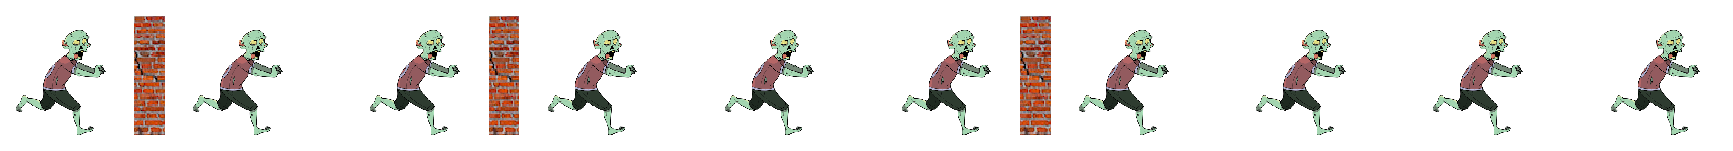
\includegraphics[scale=0.24,alt={zombies bound by walls}]{images/created/zombie_walls1.png}
    \end{center}
    where none of the groups are empty; \(1+2+3+4=10\).  Which we can also think of as 1 zombie before the first wall, 3 total before the second, 6 total before the third, and 10 altogether.
    
    
    Or, like so
    \begin{center}
        % \inputtikz{zombie_walls2}
        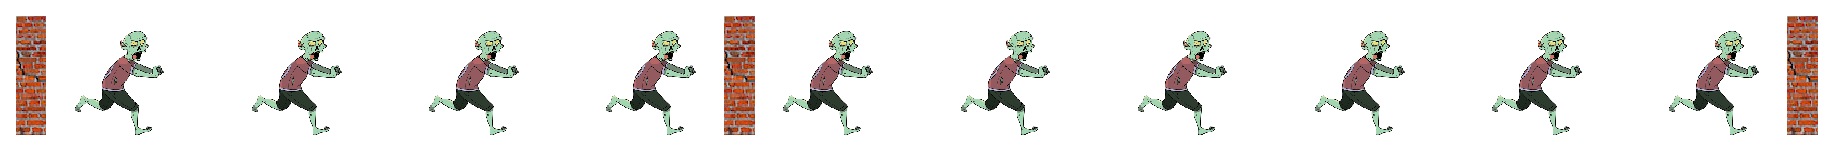
\includegraphics[scale=0.24,alt={more zombies and walls}]{images/created/zombie_walls2.png}
    \end{center}
    where the first and last groups are empty; \(0+4+6+0=10\).  Which again we can think of as 0 zombies before the first wall, 4 total before the second, and 10 total before the third, and also 10 altogether.

    Either way we need to arrange our 10 zombies and 3 walls in a row to get our 4 groupings.  Thus the total number of possible choices is
    \[\binom{r+n-1}{r}=\binom{10+4-1}{10}=\binom{13}{10}=286.\]
\end{exposition}

\begin{practiceprob}{Book Shelves}
    In how many ways can you place 23 books onto 3 shelves?\par
    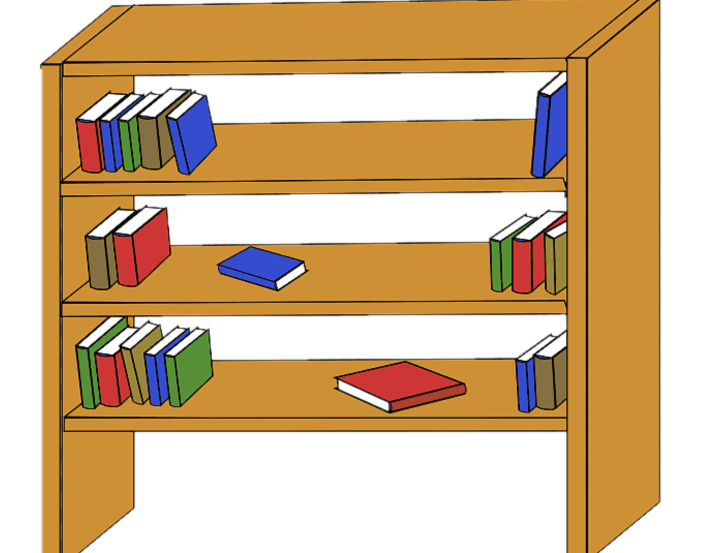
\includegraphics[height=0.13\textheight,alt={a book shelf}]{images/book_shelves.png}
\end{practiceprob}

\begin{practiceprob}{Buying Soda}
    You go to a store to buy soda for a party, if there are 5 types of soda and you need to get 48 sodas total, in how many ways can you pick out the sodas?
\vspace{0.15\textheight}
\end{practiceprob}

\clearpage

\begin{practiceprob}
    You realize that you should really make sure to have at least 6 cans of each type of soda.  With this in mind, how many ways can you now pick out sodas?
\vspace{0.19\textheight}
\end{practiceprob}

\begin{practiceprob}
    You will also need chips.  There are 3 types of chips and you want 7 bags.  However, there are only 3 bags of one of the types.  With this limitation, in how many ways can you select chips?
\vspace{0.19\textheight}
\end{practiceprob}

\begin{practiceprob}
Look at the code below and note that \(0\leq k\leq j\leq i\leq 9\), why does this code print ``Discrete Rules!!!" 220 times? (Hint: There are ten numbers to move through and three variables to assign.)

\begin{minted}{python}
count=1
for i in range(10):
    for j in range(i+1):
        for k in range(j+1):
            print("(%d) Discrete Rules!!!"%count)
            count+=1
\end{minted}

\vspace{0.17\textheight}
\end{practiceprob}